\documentclass{article}
\usepackage[utf8]{inputenc}
\usepackage{amsmath}
\usepackage{mathtools}
\usepackage{bm}
\usepackage{graphicx}
\title{COL352: Assignment 1}
\author{Sachin 2019CS10722 }
\date{January, 2022}

\begin{document}

\maketitle

\section{Question 1}

\textbf{Given an alphabet $\Gamma $ = $\{l_1,...,l_k\}$, construct an NFA that accepts strings that don't have
all the characters from $\Gamma $. Can you give an NFA with k states?}\\

\begin{enumerate}
    \item \textbf{NFA construction: }\\
Consider NFA N : $(Q, \Sigma, \delta, Q_0 , F )$ of given language, as follows:- \\
$Q =  \{s, q_{l_1}, q_{l_2}, ....... q_{l_k}\}$\\
$Q_0 = s$\\
$\Sigma = \Gamma \bigcup \{\epsilon\}$\\
$F = Q$ (all states are accepting states)\\
$\delta \subseteq Q \times \Sigma \times Q$ defined as follows:\\

\begin{equation}
    \delta (q,a) = 
    \begin{cases*}
        \{q_{l_i}\} & if $ q = q_{l_i} \text{ } \& \text{ } a \neq l_i$ \\
        \{q_{l_1}, q_{l_2} .... q_{l_k}\} & if $ q = s \text{ } \& \text{ }a = \epsilon$\\
        \phi & O.W.
    \end{cases*}
\end{equation}


\textbf{Proof of correcness: }\\
From construction it is clear that NFA N is union of k NFA's (each state $q_{l_i}$ is considering one individual NFA $N_i$).\\
Because except those $N_i$ we have one start state that has $\epsilon$ transitions to all $N_i$ (same construction of union done in lecture).\\

\textbf{Claim: } Each $N_i$ accepts only those strings that don't have the characters $l_{i}$.\\
It is easy to prove since there is only one state in $N_i$ and that too is accepting, so evey string will be accepting unless it has any character c such that $\delta(q_{l_i},c) = \phi$ and 
for every i it is only one character $l_i$\\
Hence proved that $\forall 1 \leq i \leq k : L(N_i) = (\Gamma \setminus {l_i})^{*} $\\
$=> L(N) = \bigcup L(N_i) = \bigcup (\Gamma \setminus {l_i})^{*} = $ required language.\\

\item \textbf{Can you give an NFA with k states?}\\

Since the k is arbitrary and its range is not provided in question, I'm taking it to be $k \geq 0$.\\
Proving that NFA with k states is not possible by contradiction.\\
Suppose for every such Language there exists an NFA with k states, then it would also be for k = 2.\\
So, let's try to construct one such NFA = {$(Q, \Sigma, \delta, q_0 , F )$} where,\\
$Q = \{s, q\}$\\
$\Sigma = \{l_1, l_2 \}$\\
$q_0 = s$\\
Now, $s \in F$ (since, $\epsilon $ has no characters from $\Sigma $).\\
Also, strings $l_1, l_2 \in $ L, $=> \delta(s,l_1) \bigcup F \neq \phi $ and $ \delta(s,l_2)  \bigcup F \neq \phi$.\\
And possible values of $ \delta(s,l_1) $ and $ \delta(s,l_2)$ are $\phi, \{s\}, \{q\}, \{s,q\}$\\
Clearly, they can't be $\phi$, also, $s \notin \delta(s,l_1) \bigcup \delta(s,l_2) $, as if that were the case then all the 
strings will get accepted. \\
So, either $ \delta(s,l_1) = \{q\}$ or $ \delta(s,l_2) = \{q\}$ making q an accepting state, that would make string $l_1l_2$ to get accepted 
but $l_1l_2 \notin L$\\
That is a contradiction.\\

As we have provided a k+1 state NFA in previous part, that is the best we can do with respect to number of states if only single start state is allowed. \\
If multiple start states are allowed then one can create an k-state NFA by removing start state s from above NFA and making all remainining k states 
start state.

\end{enumerate}

\pagebreak
% -------------------------------------------------
\section{Question 2}
\textbf{An all-NFA M is a 5-tuple \boldsymbol{$(Q, \Sigma, \delta, q_0 , F )$} that accepts \boldsymbol{$x \in \Sigma^{*}$} 
if every possible state that M could be in after reading input x is a state from F . Note, in contrast, that an ordinary NFA 
accepts a string if some state among these possible states is an accept state. Prove that all-NFAs recognize the class of regular languages.}\\
\\
To prove that all-NFA's recognise the class of regular languages we need to show two things, firstly that the language accepted 
by all-NFA's is regular, and secondly given any regular language there exists an all-NFA which accepts it. Following are the proofs of these parts,
\\
\\
\textbf{To Prove:} Language accepted by all-NFA is regular.\\
\textbf{Proof:} Now by the definition, all-NFA M is a 5-tuple $(Q, \Sigma, \delta, q_0 , F )$ that accepts $x \in \Sigma^{*}$ if 
every possible state that M could be in after reading input x is a state from F . This would mean the all-NFA's are NFA because NFA a
ccepts the string even if some of the states reached after reading an input x is in accept state F. NOw we know that the language 
accepted by NFA is regular. Therefore the language accepted by all-NFA is also regular. Hence proved.\\
\\
\textbf{To Prove:} For every regular language there exists an all-NFA that accepts it.\\
\textbf{Proof:} We know that for every regular language there exists a DFA which accepts it. Now the definition of a 
DFA M is that it is a 5-tuple $(Q, \Sigma, \delta, q_0 , F )$ that accepts $x \in \Sigma^{*}$ if the state that M could 
be in after reading input x is a state from F. Now we also know that the set of states DFA M would be in after reading the 
input x is a singleton set (Deterministic nature) and the state belongs to F if x is accepted by DFA. So every DFA is an
 all-NFA. Therefore for every regular language, there exists an all-NFA that accepts it. Hence proved.\\
\\
Now above two facts would imply that the all-NFA's recognize the class of regular languages.


\pagebreak
% ------------------------------------------------
\section{Question 3}

Let our regular language L can be recognized by DFA D : $(Q, \Sigma, \delta, q_0 , F )$ \\

Now, consider NFA N :  $(Q', \Sigma, \delta', q'_0 , F' )$ defined as follows:\\
$Q' = Q \bigcup \{q_{xy} \forall x \in Q, y \in  \Sigma \}$\\
$q'_0 = q_0$\\
$F = F'$\\
$\delta \subseteq Q' \times \Sigma \times Q'$ defined as follows:\\

\begin{equation}
    \delta' (q,a) = 
    \begin{cases*}
        \{q_{qa}\} & if $ q \in Q $ \\
        \{\delta(x,a)\} & if $ q = q_{xa}$\\
        \phi & O.W.
    \end{cases*}
\end{equation}
 So, basically we've added new state for each transitions in old DFA D to construct NFA N.\\

\textbf{Claim: L(D') = repeat(L)}\\
Let the run of some string s = $l_1l_2...l_k \in L$ of D is as follows (since DFA has unique run for each string, so it will be unique):- \\ \\
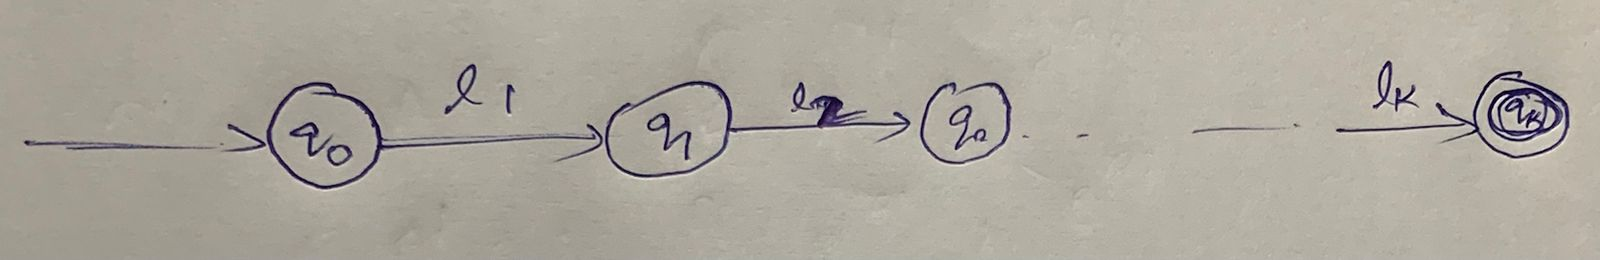
\includegraphics[width=13cm]{1.jpeg}\\
Now, one of the run of string repeat(s) = $l_1l_1l_2l_2...l_kl_k \in repeat(L)$ in N that will be parallel to above run of D will be as follows:- \\\\
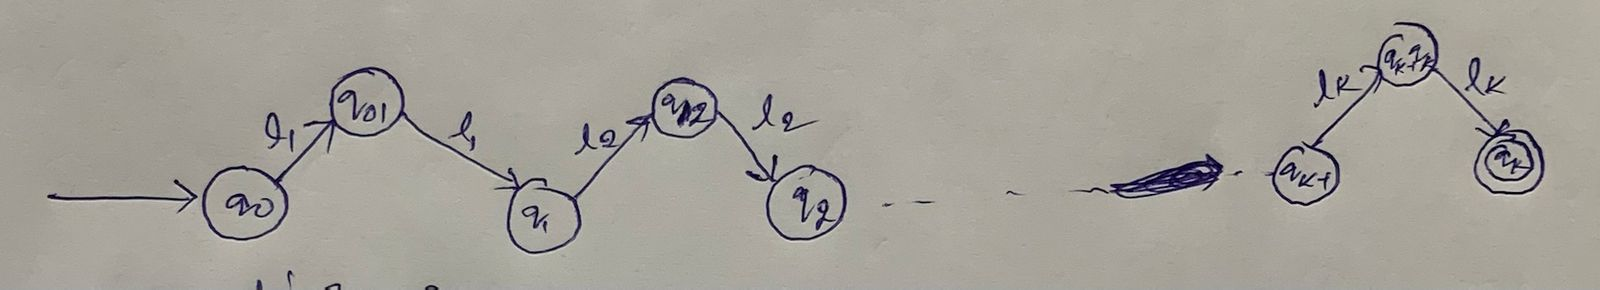
\includegraphics[width=13cm]{2.jpeg}\\

This reconstructed NFA can recognise this input sting $l_1l_!l_2l_2...l_kl_k$ if $q_k$ is accepting state it still remains accepting state after recontructing. So,regular languages are closed under repeat operation.where repeat operation is\\
$$repeat(L)=\{l_1l_1l_2l_2...l_kl_k|l_1l_2...l_k \in L \}$$\\

Let's prove this rigirously\\

\pagebreak

\textbf{Proof of correctness:}\\
Initially we took a string s = $l_1l_2...l_k \in L$ and we have run of s on D = $q_0,q_1,q_2....,q_k$
such that $q_k \in F$ and $\delta(q_i,l_{i+1})=q_{i+1}$.\\

Now, let's prove that L(N) = repeat(L) by induction.\\

\textbf{Proof by induction:(on number of characters in string)}\\

\textbf{Base case:} k = 0\\
So, s = $\epsilon $, as both D and N start from sam start state $q_0$ as have same accepting state, if D accepts $\epsilon => q_0 \in F$ then N also accepts $\epsilon$ and also vice versa.\\
Note that if $\epsilon \in L => \epsilon \in $repeart(L), as $\epsilon = \epsilon \epsilon$\\ 

\textbf{I.H.:} Let $\forall k \leq n$ N accepts only string that are of the form $l_1l_1l_2l_2...l_kl_k : l_1l_2....l_k \in L$\\

\textbf{I.S.:} Consider string s $\in \Sigma^*$ such that length of s = n+1 or n+2.
    \begin{enumerate}
        \item  $s \notin $ repeat(L)\\
        $=> $ s = $l_1l_1...l_{i-1}l_{i-1}l_il_j.... : l_1....l_i \in L$ (note that $l_{i-1}$ can be $\epsilon$ also, in that case first character itself is not repeated. This proof will work for that 
        case also)\\
        $=> $ substring $l_1l_1...l_{i-1}l_{i-1} $ will get accepted (by I.H.) and also it would have only single run in N\\
        $q_0 \xrightarrow{l_1} q_{0l_1} \xrightarrow{l_1} q_1 ....... \xrightarrow{l_{i-1}} q_{i-1}$ (as in our NFA, all transitions have $|\delta'(q,a)| \leq 1$).\\
        $q_{i-1} \xrightarrow{l_i} = \delta'(q_{i-1},l_i) = q_{(i-1)l_i} \xrightarrow{l_i} = \phi$ (since $i \neq j$)\\
        Hence rejected, that is correct as $s \notin $ repeat(L).

        \item  $s \in $ repeat(L)\\
        $=> $ s = $l_1l_1...l_nl_n : l_1....l_n \in L$\\
        By I.H., substring $l_1l_1...l_{n-1}l_{n-1}$ will be accepted.\\
        $=> q_0 \xrightarrow{l_1} q_{0l_1} \xrightarrow{l_1} q_1 ....... \xrightarrow{l_{n-1}} q_{n-1} \in F'$ 
        $q_{n-1} \xrightarrow{l_n} = \delta'(q_{n-1},l_n) = q_{(n-1)l_n} \xrightarrow{l_n} = q_n \in F $ since $l_1l_2....l_k \in L$\\
        as $F = F' => q_n \in F'$\\
        Hence accepted, that is correct as $s \in $ repeat(L).
    \end{enumerate}





\pagebreak
% ------------------------------------------------
\section{Question 4}
\textbf{Design an algorithm that takes as input the descriptions of two DFAs, D1 and D2, and
determines whether they recognize the same language}\\

Lets take two DFAs $D_1$=($Q_1$,$\Sigma$,$q_0$,$\delta_1$,$F_1$) and $D_2$=($Q_2$,$\Sigma$,$r_0$,$\delta_2$,$F_2$).\\
\textbf{Idea:}\\
Let L(d) is language recognized by dfa d.
If two DFAs will recognise same DFAs implies L($D_1$) - L($D_2$) and L($D_2$) - L($D_1$) should be a null set else language recognized by two DFAs are different.\\
\textbf{Algorithm:}\\
For computing L($D_2$)-L($D_1$):\\
\textbf{Step1(complementation)}:Generate another DFA $D_3$ which is complement of $D_2$ i.e by reversing final states as non final states and vice-versa.Then $D_3$=($Q_2$,$\Sigma$,$r_0$,$\delta_2$,\\$Q_2$-$F_2$).\\
\textbf{Step2(intersection)}:Generate another DFA $D_4$ by intersecting $D_1$ and $D_3$. Now this can be done by making a new DFA with $|Q_1|*|Q_2|$ number of states. Now the states in this dfa are touple of the states 
from the two original DFA's, first element from D1 and second from $d_3$. The start state is the touple $(s_1,s_2)$ where $s_1$ and $s_2$ are start states of $D_1$ and $D_3$
 A transtion exist between a state $(p,q)$ to $(x,y)$ on alphabet a if in original DFAs p to x and q to y transitions existed on aphabet a. 
All the touples which have either of the state as an accept state in the orginal DFA is an accept state in the new DFA.\\
\textbf{Step3(BFS)}:Perform BFS on start state of $D_4$ if it find any final state then return false else \\
\textbf{Step4}:Repeat steps 1,2,3 for computing L($D_1$)-L($D_2$) if bfs in this also finds nothing then return true.\\
\textbf{Proof of correctness:}\\
\textbf{Claim1:}Let A,B be two DFAs then if they recognise same language then the given algorithm would return true\\
\textbf{Proof by contradiction:}
Now we know that 2 language is same when both L(A)-L(B) and L(B)-L(A) are null. And when both the language is same then the DFA'a A and B recognise the same language.
Lets say L(A)-L(B) is not null then there there exist a string in L(A) which will be in L(A) and not L(B).
Now the DFA $D_4$ which we have created would accept it and hence by our algortihm false is returned. Now similary when L(B)-L(A) is not null false is retuned when doing BFS.
So our alogorithm only return true when both L(A)-L(B) and L(B)-L(A) are null. Thus our algorithm is indeed correct.\\
\textbf{Time complexity:}Worst case Time complexity of this algorithm will be O(${|Q_1|*|Q_2|}$+no of transistions in $D_4$)


\pagebreak
% ------------------------------------------------
\section{Question 5}

\textbf{For any string \boldsymbol{$w = w_1 w_2 . . . w_n$} the reverse of w written \boldsymbol{$w^R$} is the string 
\boldsymbol{$w_n . . . w_2 w_1$}. For any language A, let \boldsymbol{$A^R ={w^R | w \in A}$}. Show that if A is regular,
 then so is \boldsymbol{$A^R$}. In other words, regular languages are closed under the reverse operation.}\\
\\
As every regular language has a DFA which accepts it, let D be $(Q, \Sigma, \delta, q_0, F )$ that accepts the language
 A. Now we will construct an NFA N from this DFA. The steps of the construction are given below. We will then show that 
 the language accepted by NFA is indeed $A^R$.\\
\\
\textbf{Construction:} To construct this NFA N we will have to reverse all the edges of the DFA D. Also make the start 
state of the D as the accepting state of the N. Add $\epsilon$ transitions to the accepting states of D from a new state 
$s$ in NFA. Make $s$ the start state of the NFA.\\
So N is $(Q_1, \Sigma, \delta^{'}, q_0^{'} , F^{'} )$ such that
\begin{equation}
\begin{split}
&            Q_1=Q\cup\{s\}\\
&           F^{'}=q_0\\
&           \delta^{'}(q_1,a) = 
            \begin{cases*}
            q_2 & if $q_1 \in Q$  and  $\delta(q_2,a)=q_1$\\
            F       & if $ q_1= s$ and $a=\epsilon$\\
            \phi & O.W.
            \end{cases*}\\
&           q_0^{'}=s \\
\end{split}
\end{equation}
\textbf{To Prove:} The language accepted by N is $A^R$.\\
\textbf{Proof:} Now take any string $w_1 w_2....w_n$ from the language A. The path(path is state then alphabet taken then
 next state reached) taken by this string to accept state in D would be $q_0,w_1,q_1,w_2,q_2.....q_n,w_n,f$ where $q_i\in
  Q$ and $f\in F$. Now take the reverse of the string $w_n w_{n-1}....w_1$. There exist a path from start to accept state 
  in N as which is as follows $s,\epsilon,f,w_n,q_n,w_{n-1}.....q_1,w_1,q_0$. We know that $q_0$ is an accept state of N.
  Thus we have got an NFA that has an accepting path for any string w in $A^R$.\\
Now we have proved that for every string in A we have a accepting path in N. Now we can also similarly prove the reverse 
direction too i.e. for every string w in $A^R$ we have accepting path in D for reverse of w. The proof of this goes as 
follows:\\ Take any string $w_1 w_2....w_n$ from the language $A^R$. The pathtaken by this string to accept state in N 
would be $s,\epsilon,f,w_1,q_n,w_2.....q_1,w_n,q_)$ where $q_i\in Q$ and $f\in F$. Now take the reverse of the string $w_n 
w_{n-1}....w_1$. There exist a path from start to accept state in D as which is as follows $q_0,w_n,q_1,w_{n-1},q_2.....q_n,w_1,
f$. We know that f is an accept state of D.Thus we have got an DFA that has an accepting path for any string w in A.\\
Hence we have proved that regular languages are closed under the reverse operation. 


\pagebreak
% ------------------------------------------------
\section{Question 6}

\textbf{Let \boldsymbol{$\Sigma$} and \boldsymbol{$\Gamma$} be two finite alphabets. A function \boldsymbol{$f : \Sigma^{*} \to \Gamma^{*}$ }is called a homomorphism if
for all x,y \boldsymbol{$ \in \Sigma^{*}, f(x . y) = f(x) . f(y)$}. Observe that if f is a string homomorphism, then
\boldsymbol{$f(\epsilon) =\epsilon$}, and the values of $f(a)$ for all a \boldsymbol{$\in \Sigma$} completely determines \boldsymbol{$f$}. Prove that the class of
regular languages is closed under homomorphisms.That is, prove that if L \boldsymbol{$\subseteq \Sigma^{*} $} is a regular
language, then \boldsymbol{$f(L) = \{f(x) \in \Sigma^{*} | x \in L \}$} is regular. Try to informally describe how you
will start with a DFA for L and get an NFA for f(L).
}

\begin{enumerate}
    \item \boldsymbol{$f(\epsilon) =\epsilon$}
    
    $\forall x,y \in \Sigma^{*} f(x.y) = f(x).f(y)$ (by defination of homomorphism)\\
    take y = $\epsilon$\\
    $=> \forall x \in \Sigma^{*} f(x.\epsilon) = f(x).f(\epsilon)$\\
    $=> \forall x \in \Sigma^{*} f(x) = f(x).f(\epsilon)$\\
    but, only $f(\epsilon) \in \Gamma^{*}$ that upon concatenation with any string generate same string is $\epsilon$ only\\
    $=> f(\epsilon) =\epsilon$\\

    This, is a property of homomorphism that it maps identity elements (of the operation upon which homomorphism property is satisfyied). Here identity element with respect to an operation (say oper) is any element of the set that maps
    every element to itself upon oper.
    In our case, since $a.\epsilon = a \forall a \in \Sigma^{*} $ as well as $a.\epsilon = a \forall a \in \Gamma^{*} $, Hence $\epsilon$ is the identity element of both $\Sigma$ and $\Gamma$

    \item \textbf{values of $f(a)$ for all a \boldsymbol{$\in \Sigma$} completely determines \boldsymbol{$f$}}\\
    
    \textbf{Given: } $f(a) \text{ } \forall \text{ }  a \in \Sigma$\\
    \textbf{To find: } $f(x) \text{ } \forall \text{ }  x \in \Sigma^{*}$\\

    Let x $\in \Sigma^{*}$\\
    $=> x = a_1 a_2 ..... a_k$ where $a_i \in \Sigma $ and $k \geq 0$\\
    $=> f(x) = f(a_1 a_2 ..... a_k)$\\
    $=> f(x) = f(a_1)f(a_2)....f(a_k)$\\
    since, each $a_i \in \Sigma$ hence, they are known.\\
    $=> f(a_1)f(a_2)....f(a_k)$ is known.\\
    $=> f(x) $ is known.\\
    Hence, we can determine $f(x) \forall x \in \Sigma^{*}$

    \pagebreak
    \item \textbf{Prove that the class of regular languages is closed under homomorphisms}

    Let, L be a regular language L, to prove that regular language is closed under homomorphism it is sufficient to
    show that for any homomorphism f, f(L) is also regular.\\
    \textbf{Given:} A regular language L, A homomorphism f\\
    \textbf{To Prove:} f(L) is also regular\\
    \textbf{Proof:}

    Since, L is a regular language, we can construct a DFA (say D) for L.\\
    So, D = {$(Q, \Sigma, \delta, q_0 , F )$} such that, L(D) = L\\
    First let me define a function $g: \Gamma \to \Sigma$ as follows:\\
    $g(a) = \{ x | f(x) = a \} $\\

    Now, Consider the NFA N = {$(Q, \Gamma, \delta', q_0 , F)$} where, \\
    $\delta' \subseteq Q \times \Gamma \times Q$ defined as follows:\\
    $ \delta' (q,a) = \{ \delta (q,x) | x \in g(a) \} $\\

    Proving that L(N) = f(L) \\
    Let, $x \in f(L) => x = f(a) $ where, $a \in L$\\
    Let, $a = a_1 a_2..... a_k$\\
    $=> x = f(a_1) f(a_2) ..... f(a_k)$ \\
    Since, $a \in L = L(D) => \exists \{q_0, q_1,......,q_k\}$ where $d_i \in Q$ such that\\
    $\delta (q_i,a_{i+1}) = q_{i+1} \forall i = 0,.....,k-1$ and $q_k \in F$\\
    by defination of $\delta'$, $\delta' (q_i,f(a_{i+1})) = q_{i+1} \forall i = 0,.....,k-1$\\
    also, $F' = F => q_k \in F'$\\
    hence, N accepts x.\\
    $=> $ N accepts every string x $\in f(L) $\\
    similarly it can be shown that N rejects every string x' $ \notin f(L) $ (as run of N is parallel to D).\\
    Hence L(N) = f(L).

\end{enumerate}





\end{document}
